% Options for packages loaded elsewhere
\PassOptionsToPackage{unicode}{hyperref}
\PassOptionsToPackage{hyphens}{url}
\PassOptionsToPackage{dvipsnames,svgnames,x11names}{xcolor}
\documentclass[
  11pt]{article}
\usepackage{xcolor}
\usepackage[a4paper,margin=2.5cm]{geometry}
\usepackage{amsmath,amssymb}
\setcounter{secnumdepth}{-\maxdimen} % remove section numbering
\usepackage{iftex}
\ifPDFTeX
  \usepackage[T1]{fontenc}
  \usepackage[utf8]{inputenc}
  \usepackage{textcomp} % provide euro and other symbols
\else % if luatex or xetex
  \usepackage{unicode-math} % this also loads fontspec
  \defaultfontfeatures{Scale=MatchLowercase}
  \defaultfontfeatures[\rmfamily]{Ligatures=TeX,Scale=1}
\fi
\usepackage{lmodern}
\ifPDFTeX\else
  % xetex/luatex font selection
  \setmainfont{DejaVuSerif.ttf}[BoldFont=DejaVuSerif-Bold.ttf,ItalicFont=DejaVuSerif-Italic.ttf,BoldItalicFont=DejaVuSerif-BoldItalic.ttf]
  \setsansfont{DejaVuSans.ttf}[BoldFont=DejaVuSans-Bold.ttf,ItalicFont=DejaVuSans-Oblique.ttf,BoldItalicFont=DejaVuSans-BoldOblique.ttf]
  \setmonofont{DejaVuSansMono.ttf}[BoldFont=DejaVuSansMono-Bold.ttf,ItalicFont=DejaVuSansMono-Oblique.ttf,BoldItalicFont=DejaVuSansMono-BoldOblique.ttf]
\fi
% Use upquote if available, for straight quotes in verbatim environments
\IfFileExists{upquote.sty}{\usepackage{upquote}}{}
\IfFileExists{microtype.sty}{% use microtype if available
  \usepackage[]{microtype}
  \UseMicrotypeSet[protrusion]{basicmath} % disable protrusion for tt fonts
}{}
\makeatletter
\@ifundefined{KOMAClassName}{% if non-KOMA class
  \IfFileExists{parskip.sty}{%
    \usepackage{parskip}
  }{% else
    \setlength{\parindent}{0pt}
    \setlength{\parskip}{6pt plus 2pt minus 1pt}}
}{% if KOMA class
  \KOMAoptions{parskip=half}}
\makeatother
\usepackage{color}
\usepackage{fancyvrb}
\newcommand{\VerbBar}{|}
\newcommand{\VERB}{\Verb[commandchars=\\\{\}]}
\DefineVerbatimEnvironment{Highlighting}{Verbatim}{commandchars=\\\{\}}
% Add ',fontsize=\small' for more characters per line
\newenvironment{Shaded}{}{}
\newcommand{\AlertTok}[1]{\textcolor[rgb]{1.00,0.00,0.00}{\textbf{#1}}}
\newcommand{\AnnotationTok}[1]{\textcolor[rgb]{0.38,0.63,0.69}{\textbf{\textit{#1}}}}
\newcommand{\AttributeTok}[1]{\textcolor[rgb]{0.49,0.56,0.16}{#1}}
\newcommand{\BaseNTok}[1]{\textcolor[rgb]{0.25,0.63,0.44}{#1}}
\newcommand{\BuiltInTok}[1]{\textcolor[rgb]{0.00,0.50,0.00}{#1}}
\newcommand{\CharTok}[1]{\textcolor[rgb]{0.25,0.44,0.63}{#1}}
\newcommand{\CommentTok}[1]{\textcolor[rgb]{0.38,0.63,0.69}{\textit{#1}}}
\newcommand{\CommentVarTok}[1]{\textcolor[rgb]{0.38,0.63,0.69}{\textbf{\textit{#1}}}}
\newcommand{\ConstantTok}[1]{\textcolor[rgb]{0.53,0.00,0.00}{#1}}
\newcommand{\ControlFlowTok}[1]{\textcolor[rgb]{0.00,0.44,0.13}{\textbf{#1}}}
\newcommand{\DataTypeTok}[1]{\textcolor[rgb]{0.56,0.13,0.00}{#1}}
\newcommand{\DecValTok}[1]{\textcolor[rgb]{0.25,0.63,0.44}{#1}}
\newcommand{\DocumentationTok}[1]{\textcolor[rgb]{0.73,0.13,0.13}{\textit{#1}}}
\newcommand{\ErrorTok}[1]{\textcolor[rgb]{1.00,0.00,0.00}{\textbf{#1}}}
\newcommand{\ExtensionTok}[1]{#1}
\newcommand{\FloatTok}[1]{\textcolor[rgb]{0.25,0.63,0.44}{#1}}
\newcommand{\FunctionTok}[1]{\textcolor[rgb]{0.02,0.16,0.49}{#1}}
\newcommand{\ImportTok}[1]{\textcolor[rgb]{0.00,0.50,0.00}{\textbf{#1}}}
\newcommand{\InformationTok}[1]{\textcolor[rgb]{0.38,0.63,0.69}{\textbf{\textit{#1}}}}
\newcommand{\KeywordTok}[1]{\textcolor[rgb]{0.00,0.44,0.13}{\textbf{#1}}}
\newcommand{\NormalTok}[1]{#1}
\newcommand{\OperatorTok}[1]{\textcolor[rgb]{0.40,0.40,0.40}{#1}}
\newcommand{\OtherTok}[1]{\textcolor[rgb]{0.00,0.44,0.13}{#1}}
\newcommand{\PreprocessorTok}[1]{\textcolor[rgb]{0.74,0.48,0.00}{#1}}
\newcommand{\RegionMarkerTok}[1]{#1}
\newcommand{\SpecialCharTok}[1]{\textcolor[rgb]{0.25,0.44,0.63}{#1}}
\newcommand{\SpecialStringTok}[1]{\textcolor[rgb]{0.73,0.40,0.53}{#1}}
\newcommand{\StringTok}[1]{\textcolor[rgb]{0.25,0.44,0.63}{#1}}
\newcommand{\VariableTok}[1]{\textcolor[rgb]{0.10,0.09,0.49}{#1}}
\newcommand{\VerbatimStringTok}[1]{\textcolor[rgb]{0.25,0.44,0.63}{#1}}
\newcommand{\WarningTok}[1]{\textcolor[rgb]{0.38,0.63,0.69}{\textbf{\textit{#1}}}}
\usepackage{longtable,booktabs,array}
\usepackage{calc} % for calculating minipage widths
% Correct order of tables after \paragraph or \subparagraph
\usepackage{etoolbox}
\makeatletter
\patchcmd\longtable{\par}{\if@noskipsec\mbox{}\fi\par}{}{}
\makeatother
% Allow footnotes in longtable head/foot
\IfFileExists{footnotehyper.sty}{\usepackage{footnotehyper}}{\usepackage{footnote}}
\makesavenoteenv{longtable}
\setlength{\emergencystretch}{3em} % prevent overfull lines
\providecommand{\tightlist}{%
  \setlength{\itemsep}{0pt}\setlength{\parskip}{0pt}}
\usepackage{tikz}
\usetikzlibrary{arrows.meta,positioning,shapes.geometric}
\usepackage{etoolbox}
\AtBeginEnvironment{longtable}{\footnotesize}
\setcounter{secnumdepth}{0}
\setcounter{tocdepth}{2}
\renewcommand{\contentsname}{Contents}
\sloppy
\setlength{\parskip}{2pt}
\newcommand{\Needspace}[1]{%
  \par
  \ifdim\pagegoal>\pagetotal
    \ifdim\dimexpr\pagegoal-\pagetotal\relax<#1\relax
      \newpage
    \fi
  \fi
}
\AtBeginDocument{\hypersetup{pdftitle={Sovereign Epistemic Acquisition: A Conditional Framework and Synthetic Audit Artifacts},pdfauthor={Wen Hu; Xutong Wang; Ya Yu},pdfkeywords={SEA; SAP; epistemic sovereignty; weighted omission}}}
\usepackage{bookmark}
\IfFileExists{xurl.sty}{\usepackage{xurl}}{} % add URL line breaks if available
\urlstyle{same}
\hypersetup{
  colorlinks=true,
  linkcolor={NavyBlue},
  filecolor={Maroon},
  citecolor={Blue},
  urlcolor={NavyBlue},
  pdfcreator={LaTeX via pandoc}}

\author{}
\date{22 November 2026}

\begin{document}

\section{\texorpdfstring{Sovereign Epistemic Acquisition:\newline A
Conditional Framework and Synthetic Audit
Artifacts}{Sovereign Epistemic Acquisition:A Conditional Framework and Synthetic Audit Artifacts}}\label{sovereign-epistemic-acquisitiona-conditional-framework-and-synthetic-audit-artifacts}

\textbf{Wen Hu}1,2~~\textbf{Xutong Wang}1~~\textbf{Ya Yu}1

1 College of Electronic and Information Engineering, Nanjing University
of Aeronautics and Astronautics, Nanjing, China\\
2 Jiangsu Yunhefeng Intelligent Technology Co., Ltd., Jiangsu, China

Corresponding author: Wen Hu (huwen@nuaa.edu.cn)

November 2026 · Human--AI collaboration; independent human mathematical
review remains pending

\begin{center}\rule{0.5\linewidth}{0.5pt}\end{center}

\subsection{Abstract}\label{abstract}

Active retrieval, passive filtering, and authority over the
recommendation objective are usually modeled separately. This paper
proposes a conditional \textbf{Sovereign Acquisition Problem (SAP)}
framework connecting pull/push actions, multi-resource budgets,
authorized objective writes and rollback, versioned target construction
under exogenous frozen evaluation-protocol events, and terminal
consumption accounting. The contribution is one conditional framework
and two checkable artifacts: a governance-conformance reference with a
minimal longitudinal synthetic executor, and a falsifiable
staged-omission audit and future-evaluation specification. Standard
dynamic-programming, value-of-information, submodular, threshold, and
KKT results are conditional technical foundations, not new general
theorems. The executor runs a declared fixture through objective
write/rollback, five resource coordinates, operational attendance
measurement, protocol registry transitions with single-line control
sealing, and an operational omission ledger; it does not establish
deployment effectiveness. Historical replay records contain only
selected proxies, so retrospective sensitivity audits are reported
without treating positive estimates or intervals as structural benefit.
The future protocol separates latent actual consumption, operational
attendance, and an all-assigned failure-composite endpoint, and gives
arm-specific bounds for operational attendance omission---not latent
consumption without measurement-error assumptions. Independent
mathematical review, third-party reproduction, matched real-model
experiments, and human data remain pending.

\textbf{Keywords}: epistemic sovereignty; active acquisition;
information filtering; governance audit; weighted omission; measurement
protocol

\section{Part I Framework and
Artifacts}\label{part-i-framework-and-artifacts}

\subsection{1 Introduction}\label{introduction}

\subsubsection{1.1 Budget and ownership}\label{budget-and-ownership}

A bounded agent cannot consume every candidate. If 45 minutes are
available and each substantive item requires at least four minutes, at
most 11 items can be consumed; in a stylized stream of \(10^4\)
candidates the discarded fraction is at least
\(1-45/(4\times10^4)=0.998875\). This is arithmetic, not a measured
universal constant. Notification and personal-information-management
research motivates the burden but does not validate this daily count for
every user (Pielot, Church \& de Oliveira, 2014; Bergman \& Whittaker,
2016).

Two design questions follow. First, how should active acquisition and
passive filtering compete for the same limited resources? Second, who
may read, write, roll back, and audit the objective against which
candidates are selected? User-controlled recommendation, preference
elicitation, contestability, and value-sensitive design already address
parts of the second question (Harper et al., 2015; Jugovac \& Jannach,
2017; Hirsch et al., 2017; Friedman \& Hendry, 2019; Santoni de Sio \&
van den Hoven, 2018). SEA does not claim to invent objective control.
Its narrower proposal is to make the ownership interface, resource
accounting, and terminal consumption event explicit in one conditional
model.

\subsubsection{1.2 One framework and two
artifacts}\label{one-framework-and-two-artifacts}

The paper makes three bounded contributions.

\begin{enumerate}
\def\labelenumi{\arabic{enumi}.}
\tightlist
\item
  \textbf{A conditional SAP framework with consumption-aligned
  omission.} Section 3 defines a finite-horizon controlled model with
  observable histories, resource-feasible and guard-admissible actions,
  authorized objective transitions, exogenous protocol-governed target
  registries, and reference-corpus availability. Section 4 defines
  weighted expected omission and separates latent actual consumption,
  operational attendance, and failure-composite measurement failure.
\item
  \textbf{A governance reference and minimal longitudinal executor.}
  Section 3 also specifies S1--S4 conformance properties and a small
  synthetic executor that runs raw candidates through update, linkage,
  selection, delivery, opening, operational attendance, resource
  deduction, objective write/rollback, and a domain-separated hash
  ledger. This is an implementation artifact, not a general SAP
  optimizer or a validated system.
\item
  \textbf{A falsifiable audit and future-evaluation specification.}
  Sections 6--7 freeze retrospective selected-proxy sensitivities, state
  what they cannot identify, and specify one future matched comparison
  with one failure-composite primary outcome, attendance-instrument
  registration, and arm-specific missing-outcome bounds.
\end{enumerate}

The following are not claimed: a globally optimal SAP algorithm; a new
general KKT, submodular, Hoeffding, Clopper--Pearson, or
dynamic-programming theorem; actual-consumption observations in the
historical replay; a deployment recall guarantee; or evidence that SEA
improves human welfare. Standard results are collected as conditional
technical foundations in Section 5 and the supplement.

\subsubsection{1.3 Claim conventions and
terminology}\label{claim-conventions-and-terminology}

A \textbf{formal result} is a derivation under stated assumptions. A
\textbf{design rule} is an engineering or normative choice. A
\textbf{synthetic implementation run} checks executable interfaces on
declared fixtures. A \textbf{retrospective sensitivity audit} summarizes
frozen historical artifacts without identifying a structural effect. A
\textbf{confirmatory experiment} would require public preregistration,
independent environments, matched baselines, and immutable analysis;
none is reported here.

Three consumption terms are kept separate throughout:

\begin{itemize}
\tightlist
\item
  \textbf{Latent actual consumption} \(D\): the theoretical terminal
  event used by the SAP reward and omission estimand. It is not directly
  observed in the historical replay or by opening receipts.
\item
  \textbf{Operational attendance} \(Z\): a validated behavioral
  measurement produced by a frozen instrument. It is evidence about
  consumption, not comprehension, learning, or latent cognition.
\item
  \textbf{Failure-composite omission} \(Y^{FC}\): an operational
  endpoint equal to one unless a valid positive operational-attendance
  measurement is obtained. Unknown terminal measurements enter this
  endpoint as failure without being rewritten as observed
  non-consumption.
\end{itemize}

Machine-to-machine events are called \textbf{machine
ingestion-and-task-reference}
(\texttt{machine\_ingestion\_and\_task\_reference}), not human
attention. They can show that content entered a declared task context
and was referenced by a task operation; they do not by themselves show
downstream information use.

\subsection{2 Related Work and Precise
Positioning}\label{related-work-and-precise-positioning}

The literature update is a structured narrative positioning with
targeted bibliographic verification, not a systematic review. Search
concepts, representative queries, publisher/ACL/NeurIPS/arXiv/Crossref
records, inclusion rules, and access dates are archived in
\texttt{docs/LITERATURE\_SEARCH\_v1.16.md}. AI-assisted search and
author revision selected sources; there was no independent dual
screening. Earlier searches did not preserve complete hit and
deduplication counts, so none are invented.

Search economics, optimal stopping, information foraging, Bayesian
experimental design, active learning, bandits, and rational inattention
supply pull-side foundations (Stigler, 1961; Weitzman, 1979; Pirolli \&
Card, 1999; Lindley, 1956; Chaloner \& Verdinelli, 1995; Settles, 2009;
Gittins, 1979; Whittle, 1988; Sims, 2003; Matějka \& McKay, 2015;
Maćkowiak, Matějka \& Wiederholt, 2023). Blackwell (1953) gives the
correctly specified information-value benchmark. Selective prediction
and cascade ranking formalize abstention and cheap-stage filtering
(Chow, 1970; Geifman \& El-Yaniv, 2017; Wang, Lin \& Metzler, 2011).
Retrieval evaluation and RAG work make upstream recall, grounding, and
answer quality distinct (Voorhees, 1998; Lewis et al., 2020; Es et al.,
2024; Saad-Falcon et al., 2024). Diversified retrieval and submodular
summarization supply coverage objectives and inherited greedy guarantees
(Carbonell \& Goldstein, 1998; Santos, Macdonald \& Ounis, 2010; Dang \&
Croft, 2012; Lin \& Bilmes, 2011; Nemhauser, Wolsey \& Fisher, 1978;
Krause, Singh \& Guestrin, 2008; Leskovec et al., 2007; Sviridenko,
2004). Misspecified-learning research studies acting under a wrong model
(Berk, 1966; Esponda \& Pouzo, 2016; Fudenberg, Romanyuk \& Strack,
2017). Agentic recommendation and proactive-assistant roadmaps
substantially weaken broad novelty claims about integrating tools,
planning, and proactivity (Peng et al., 2025; Lin et al., 2026).
Welfare-oriented recommendation and human-values synthesis supply the
adjacent objective-side motivation (Allcott et al., 2020; Stray et al.,
2024).

Table 1 compares the closest traditions on the specific interfaces
claimed here. ``Defined'' means specified in this paper; ``implemented''
means present in the synthetic reference; ``validated'' would require an
experiment, and no row is experimentally validated for deployment
effectiveness. Because the review is non-exhaustive, negative cells use
\textbf{NC} = not central in the cited representative works, and
\textbf{NI} = not identified in the reviewed sources; they are not
universal claims about entire literatures.

\textbf{Table 1. Interface comparison with closest traditions.}

\begin{longtable}[]{@{}
  >{\raggedright\arraybackslash}p{(\linewidth - 12\tabcolsep) * \real{0.1429}}
  >{\raggedright\arraybackslash}p{(\linewidth - 12\tabcolsep) * \real{0.1429}}
  >{\raggedright\arraybackslash}p{(\linewidth - 12\tabcolsep) * \real{0.1429}}
  >{\raggedright\arraybackslash}p{(\linewidth - 12\tabcolsep) * \real{0.1429}}
  >{\raggedright\arraybackslash}p{(\linewidth - 12\tabcolsep) * \real{0.1429}}
  >{\raggedright\arraybackslash}p{(\linewidth - 12\tabcolsep) * \real{0.1429}}
  >{\raggedright\arraybackslash}p{(\linewidth - 12\tabcolsep) * \real{0.1429}}@{}}
\toprule\noalign{}
\begin{minipage}[b]{\linewidth}\raggedright
Tradition
\end{minipage} & \begin{minipage}[b]{\linewidth}\raggedright
Explicit objective-write authorization
\end{minipage} & \begin{minipage}[b]{\linewidth}\raggedright
Version rollback
\end{minipage} & \begin{minipage}[b]{\linewidth}\raggedright
Unified pull/push multi-resource budget
\end{minipage} & \begin{minipage}[b]{\linewidth}\raggedright
Fixed-supply vs supply-ecology separation
\end{minipage} & \begin{minipage}[b]{\linewidth}\raggedright
Terminal consumption rather than click/selection
\end{minipage} & \begin{minipage}[b]{\linewidth}\raggedright
Status here
\end{minipage} \\
\midrule\noalign{}
\endhead
\bottomrule\noalign{}
\endlastfoot
Search, foraging, bandits, rational inattention & NC & NC & Often
single-resource or index-specific & NI & Usually reward/selection, not
audited consumption & Borrowed components \\
User-controlled and welfare recommendation & User configuration exists &
NI & Not a common pull/push budget & NI & Engagement/welfare proxies
vary & Adjacent, not replaced \\
MMR, xQuAD, PM-2, submodular summarization & NI & NI & Selection cost
only & NI & Selection/summary quality & Inherited algorithms \\
RAG and agentic recommendation & Tool permissions, not objective-store
guard & NI & Token/latency budgets, not unified SAP & NI &
Context/answer proxies & Architectural comparator \\
Misspecified learning & NC & NC & NC & NC & Decision utility, not
consumption audit & Upstream theory \\
Human control, contestability, VSD & Normative control principles & NI &
NC & NI & Human outcomes, not this ledger & Governance motivation \\
SEA conditional framework & Defined and synthetically implemented &
Defined and synthetically implemented & Defined; five coordinates in
executor & Defined and synthetically tested & Defined; operational
attendance measured only in fixtures & Framework + artifacts, not
effectiveness \\
\end{longtable}

The conjunction is the claimed contribution, not any single cell. The
table does not assert that no prior system has any of these properties;
it states what the cited representative traditions establish and what
this paper adds as a conditional specification.

\subsection{3 The Conditional SAP Framework and Reference
Artifacts}\label{the-conditional-sap-framework-and-reference-artifacts}

\subsubsection{3.1 Target construction, availability, and
versioning}\label{target-construction-availability-and-versioning}

An information item \(x_i\) is mapped by a versioned target map
\(\mathcal T_v:x_i\mapsto 2^{E_v}\) to zero or more propositions in a
target registry \(v\). A proposition is not automatically a document,
company--day, or event. The registry must contain canonical proposition
text, construction evidence, target weights, a reference-corpus
snapshot, and candidate--target availability evidence. Availability is
relative to that frozen reference universe: a closed snapshot can
support ``unavailable in this snapshot,'' but not open-world
nonexistence. Each reference document declares
\texttt{first\_available\_period}; the executor treats availability as
persistent from that period onward and filters longitudinal eligibility
by period.

Dynamic target sets separate \textbf{control continuity} from
\textbf{evaluation cohorts}. A target-set or mapping version change
creates a new evaluation cohort
(\texttt{NEW\_EVALUATION\_COHORT\_\_NO\_CROSS\_VERSION\_POOLING});
estimates are not pooled across versions. Version changes are
\textbf{exogenous evaluation-protocol events, not policy actions}: the
protocol freezes a finite registry family, an ordered version schedule,
and a switch timing (\texttt{switch\_after\_period} per scheduled
successor) before the run and before any arm result is read, and the
control instance follows that schedule along a single active control
path. At a protocol transition, accepted only at the declared period
boundary, the preceding control path is sealed, so objective,
authorization, rollback, audit, and resource state remain unique; a full
reset starts a new control instance as a declared protocol exception,
selecting a pre-declared allowed reset target and generating a fresh
independent schedule, not a theorem about SAP control. Section 3.2 makes
this explicit in the tuple: the active registry is part of state, and
each cohort evaluates under its own measure \(\nu^{(v)}\). Merge/split
changes are estimand changes unless weights, mapping, and terminal
events are jointly aligned.

A small synthetic target-construction audit is provided in
\texttt{sim/sea\_sap/target\_construction.py}. It reports agreement
between two deterministic extraction rules, a frozen arbitration rule,
and a merge/split sensitivity example. In that fixture, fine-grained
weighted omission is 0.5 while a coarse ANY-member grouping gives 1/6.
This demonstrates non-invariance under granularity; it is not human
annotation. Independent human target validation remains pending, and a
blank blinded annotation template is included.

\textbf{Table 2. Measurement and target objects.}

\begin{longtable}[]{@{}
  >{\raggedright\arraybackslash}p{(\linewidth - 6\tabcolsep) * \real{0.2500}}
  >{\raggedright\arraybackslash}p{(\linewidth - 6\tabcolsep) * \real{0.2500}}
  >{\raggedright\arraybackslash}p{(\linewidth - 6\tabcolsep) * \real{0.2500}}
  >{\raggedright\arraybackslash}p{(\linewidth - 6\tabcolsep) * \real{0.2500}}@{}}
\toprule\noalign{}
\begin{minipage}[b]{\linewidth}\raggedright
Object
\end{minipage} & \begin{minipage}[b]{\linewidth}\raggedright
Meaning
\end{minipage} & \begin{minipage}[b]{\linewidth}\raggedright
How obtained
\end{minipage} & \begin{minipage}[b]{\linewidth}\raggedright
What it is not
\end{minipage} \\
\midrule\noalign{}
\endhead
\bottomrule\noalign{}
\endlastfoot
Target registry \(v\) & Versioned proposition set, weights, map
\(\mathcal T_v\) & Frozen construction rule, evidence, reference
snapshot & A universal complete target set \\
Reference availability \(A^{ref}\) & Item supports target in frozen
reference corpus & Content hash, source pointer, first available period
& Open-world existence or truth \\
Latent consumption \(D\) & Theoretical terminal consumption event & Not
directly observed here & Opening, dwell, or machine receipt \\
Operational attendance \(Z\) & Validated behavioral measurement & Frozen
instrument, thresholds, blind adjudication & Comprehension, learning,
welfare \\
Machine ingestion-and-task-reference & Synthetic placeholder for
content/receipt/task binding & Fixture hash strings; real logs need
bound evidence & Human attention, downstream information use, or
cryptographic proof \\
Failure-composite \(Y^{FC}\) & No valid positive operational attendance
& Preregistered endpoint rule & Latent omission \(\mathcal M_\nu\) \\
\end{longtable}

\subsubsection{3.2 Finite-horizon SAP
tuple}\label{finite-horizon-sap-tuple}

A conditional SAP instance is defined \textbf{per control instance}: the
active target registry is part of state, registry-version transitions
are exogenous frozen evaluation-protocol events rather than policy
actions, and the evaluation measure is selected per cohort from a
declared version-indexed family (the dynamic-target closure):

\[\mathrm{SAP}=\langle H,\gamma,\mathcal X,\mathcal Y,\widetilde{\mathcal A},\{\mathcal A_t\},P,r,\Phi,\mu_0,\mathcal G,\{\nu^{(v)}\}_{\rho^{(v)}\in\mathfrak R}\rangle.\tag{1}\]

\begin{itemize}
\tightlist
\item
  \textbf{Horizon.} \(t=0,\ldots,H\), \(H<\infty\), \(\gamma\in(0,1]\).
  The initial law \(\mu_0(x_0,y_0)\) gives \(h_0=(y_0)\). Conditional
  history laws are used only on positive-probability support.
\item
  \textbf{State.}
  \(x_t=(s_t,\vartheta_t,\mathcal V_t,Q_t,B_t,L_t,\chi_t,\rho_t)\). Here
  \(s_t\) contains environment, candidate, user, and producer states;
  \(\vartheta_t\) is the objective store; \(\mathcal V_t\) is
  append-only objective version history; \(Q_t\) contains queues;
  \(B_t\) is the remaining resource vector; \(L_t\) is the audit ledger;
  \(\chi_t\) contains public/emergency state; and
  \(\rho_t=(v_t,E_{v_t},\mathcal T_{v_t},A^{ref}_{v_t})\) is the active
  frozen target registry: version, proposition set, candidate--target
  map, and reference-availability evidence. The registry family
  \(\mathfrak R=\{\rho^{(1)},\ldots,\rho^{(K)}\}\) is finite and
  declared ex ante with content hashes; \(K=|\mathfrak R|\).
\item
  \textbf{Observation.} \(y_t\) contains source/query responses, budget
  observations, authorization receipts, delivery/opening/attendance
  receipts when measured, and audit observations. The policy information
  is \(h_t=(y_0,a_0,\ldots,a_{t-1},y_t)\); latent states are not policy
  inputs.
\item
  \textbf{Action sets.} Attempted actions \(a_t\) include monitoring,
  pull, push, delivery, objective write/rollback, and override;
  registry-version transitions are \textbf{not} policy actions (below).
  Let \(\mathcal A^{res}_t(h)\) be resource-feasible actions,
  \(\mathcal A^{att}_t(h)\) syntactically valid loggable attempts, and
  \(\mathcal A^{guard}_t(h)\) guard-admissible attempts. The policy
  chooses from
  \(\mathcal A_t(h)=\mathcal A^{att}_t(h)\cap\mathcal A^{res}_t(h)\).
  Unauthorized but canonical write attempts remain in
  \(\mathcal A^{att}_t\) so rejection can be logged; they are not
  silently removed from the action space. Guard acceptance is a
  transition constraint, not a reason to erase the attempt.
\item
  \textbf{Budgets.}
  \(B_t=(B_t^T,B_t^{cmp},B_t^{call},B_t^{\$},B_t^{risk})\) records time,
  computation, model/tool call units, money, and authorized risk. A
  resource-feasible action satisfies \(0\le c(x_t,a_t)\le B_t\)
  componentwise and \(B_{t+1}=B_t-c(x_t,a_t)+\zeta_t\), with declared
  replenishment \(\zeta_t\).
\item
  \textbf{Exogenous registry transitions and evaluation cohorts.} The
  evaluation protocol declares ex ante the finite frozen family
  \(\mathfrak R\), an ordered version schedule, and a frozen switch
  timing (\texttt{switch\_after\_period} per scheduled successor), all
  fixed before any arm result is read. A registry-version transition
  replaces \(\rho_t\) by the next scheduled family member, content-hash
  verified, only when exactly the declared number of periods has
  completed, and appends a cohort-boundary record to \(L_t\). It is an
  evaluation-protocol event outside every \(\mathcal A_t\): the policy
  cannot switch registries, and no objective-write authorization is
  required or meaningful for it, because it is not a policy action;
  protocol membership/schedule/timing validation replaces authorization
  here. The control lifecycle is \textbf{single-line}: at a transition
  the preceding control path is sealed and can no longer act, the
  successor is the unique active path of the same control instance, and
  objective, authorization, audit, and resource state are shared as one
  unique state, never copied into parallel branches. Continuity
  transitions strictly advance along the schedule; a full reset is a
  declared exception for an independent control instance, selecting a
  pre-declared allowed reset target from the family (backward versions
  or members outside the parent schedule only if declared) and
  generating a fresh independent single-version schedule; it is never a
  registry rollback of the sealed parent. An \textbf{evaluation cohort}
  is a maximal interval of constant \(v_t\) along the single path. Its
  estimand uses \(\nu^{(v_t)}\), chosen at evaluation time from the
  declared family rather than fixed permanently as a control parameter;
  estimates are never pooled across cohorts. There is no registry
  rollback, and objective rollback restores an objective version only,
  never a registry version.
\item
  \textbf{Reward.} For authorized \(\vartheta_t\),
  \(r_t=r^{dec}_{\vartheta_t}(s_t,a_t,D_t)+r^{ref}_{\vartheta_t}(s_t,a_t)-\sum_\ell\lambda_{\ell,t}h_{\ell,t}(s_t,a_t)\),
  with terminal cost \(\Phi(x_{H+1})\). Decision reward uses latent
  consumption \(D_t\), not selection. The target measure entering the
  omission estimand at time \(t\) is \(\nu^{(v_t)}\). A policy \(\pi\)
  induces
\end{itemize}

\[J(\pi)=\mathbb E^\pi\!\left[\sum_{t=0}^{H}\gamma^t r_t-\gamma^{H+1}\Phi(x_{H+1})\right].\tag{2}\]

The tuple closes a conditional problem statement; it does not make the
problem tractable---optimal queueing-network control is already
computationally hard (Papadimitriou \& Tsitsiklis, 1999)---or identify
personal utility. Because the registry family is finite and frozen ex
ante and transitions follow the fixed protocol schedule and switch
timing, adding \(\rho_t\) to state preserves the finite-history
existence argument (Proposition 3.1; Supplement SA.0). Figure 1 shows
the information and authorization flow.

\begin{figure}[htbp]
\centering
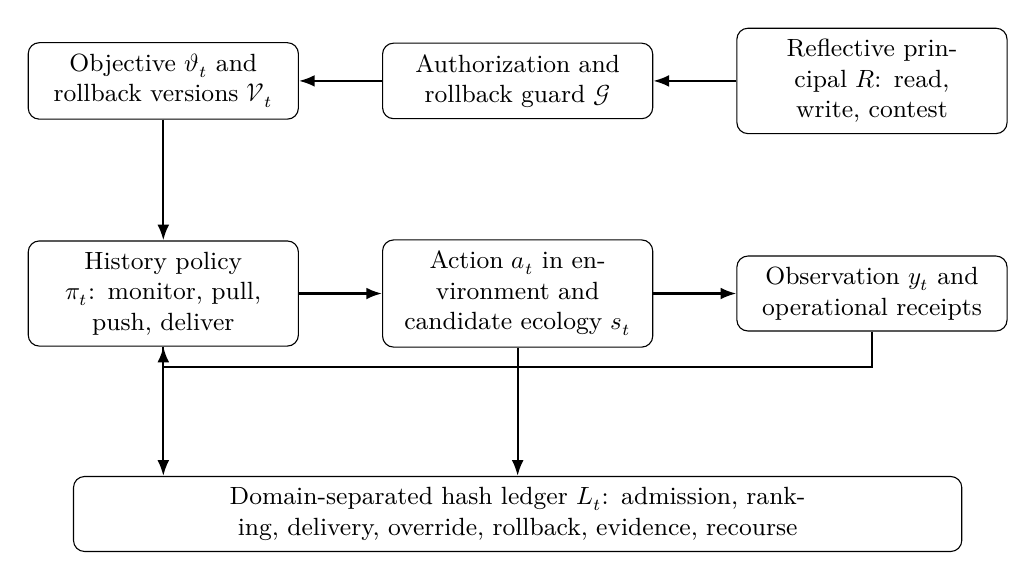
\begin{tikzpicture}[font=\small,
 box/.style={draw,rounded corners,align=center,inner sep=4pt,text width=3.15cm},
 arr/.style={-{Latex[length=2mm]},thick}]
\node[box] (store) at (0,0) {Objective $\vartheta_t$ and rollback versions $\mathcal V_t$};
\node[box] (auth) at (4.5,0) {Authorization and rollback guard $\mathcal G$};
\node[box] (principal) at (9,0) {Reflective principal $R$: read, write, contest};
\node[box] (policy) at (0,-2.7) {History policy $\pi_t$: monitor, pull, push, deliver};
\node[box] (env) at (4.5,-2.7) {Action $a_t$ in environment and candidate ecology $s_t$};
\node[box] (obs) at (9,-2.7) {Observation $y_t$ and operational receipts};
\node[box,text width=11cm] (ledger) at (4.5,-5.5) {Domain-separated hash ledger $L_t$: admission, ranking, delivery, override, rollback, evidence, recourse};
\draw[arr] (principal) -- (auth);
\draw[arr] (auth) -- (store);
\draw[arr] (store) -- (policy);
\draw[arr] (policy) -- (env);
\draw[arr] (env) -- (obs);
\draw[arr] (obs.south) -- ++(0,-0.45) -| (policy.south);
\draw[arr] (policy.south) -- (ledger.north -| policy);
\draw[arr] (env.south) -- (ledger.north -| env);
\end{tikzpicture}
\caption{SAP information flow. Platform variables may affect candidate ecology, but objective changes pass through the authorization guard. Registry-version transitions are exogenous protocol events outside the policy action set, following the frozen family $\mathfrak R$, schedule, and switch timing. The ledger records both paths separately, including cohort boundaries and control-path sealing.}
\label{fig:sap-flow}
\end{figure}

\subsubsection{3.3 Guarded transitions and the exact audit hash
specification}\label{guarded-transitions-and-the-exact-audit-hash-specification}

For a write proposal \((\vartheta^+,\sigma_R)\), the guard checks
actor--principal consistency, the operation identifier (which is the
scope of this reference guard), exact proposal hash, current version
token, single-use authorization ID, and monotonic structural timestamp.
Period-\(t\) ranking, delivery, and reward use the pre-write
\(\vartheta_t\); guard processing occurs after those decisions. Accepted
writes append a new current version; rollback restores an identified
version as a newly appended current version. Rejected canonical attempts
leave the objective unchanged apart from the rejection record. The guard
governs objective writes and rollback only. Registry transitions are not
guard operations: the executor instead validates them against the frozen
protocol declaration (family membership, content hash, next scheduled
position, frozen switch timing, declaration integrity, active-path
status), and rejected non-family, tampered, out-of-schedule, mistimed,
declaration-tampered, or sealed-path attempts leave the registry,
objective store, budget, and active path unchanged; the only state
change is one appended rejection audit record in \(L_t\), with zero
resource spend. Objective rollback and registry version are independent:
rollback never restores a registry version.

The implementation uses domain-separated canonical JSON, not recursive
embedding of the previous record. Let

\[b_{t+1}=(\mathrm{schema},\mathrm{sequence},\mathrm{event},\mathrm{timestamp},\mathrm{evidence},\mathrm{payload},H_t),\]

and let
\(J_{t+1}=\{\mathrm{domain}:\texttt{sea-governance-record/2},\mathrm{value}:b_{t+1}\}\).
Then

\[r_{t+1}=(b_{t+1},H_{t+1}),\qquad H_{t+1}=\mathrm{SHA256}\bigl(\mathrm{canonical}(J_{t+1})\bigr).\tag{3}\]

The genesis hash is 64 zero characters. Canonical JSON sorts object
keys, uses UTF-8, compact separators, and rejects non-finite floats.
Hash chaining detects edits relative to retained records and an external
anchor; it is not consensus, authenticated identity, or protection
against a host that replaces the whole store and anchor.

\textbf{Proposition 3.1 (Finite observable-history existence).}
\emph{Under finite horizon, finite primitive actions/observations,
finite latent exogenous range, bounded rewards and terminal cost, and a
nonempty finite resource-feasible loggable attempt set at each history,
an optimal deterministic history-dependent policy exists.}

The proof is a standard finite-history dynamic-programming argument. Fix
a full-support behavioral reference policy \(\beta\), for example
uniform over each nonempty feasible attempt set. Conditional rewards,
next-observation kernels, and terminal costs are defined on
positive-\(\beta\)-probability histories. At a history with zero
probability under \(\beta\)---and therefore under every policy---assign
any fixed feasible action and finite continuation value; such
assignments cannot affect reachable values. The Bellman maximum is
attained over a finite set. Full details are in Supplementary Appendix
SA.0. This is not a tractable algorithm or a low-dimensional
belief-sufficiency result.

\Needspace{30em}

\subsubsection{3.4 Algorithm 1 and the minimal longitudinal
executor}\label{algorithm-1-and-the-minimal-longitudinal-executor}

Algorithm 1 is an \textbf{audit schedule and synthetic executor
interface}, not a globally optimal SAP solver.

\begin{Shaded}
\begin{Highlighting}[]
\NormalTok{Input: history h, objective θ, versions V, budgets B,}
\NormalTok{       raw candidates X, active protocol registry ρ\_t, instrument registry}
\NormalTok{ 0  Whole{-}period resource precheck and commit{-}free selection dry run;}
\NormalTok{    reject infeasible terminal plans before any state mutation.}
\NormalTok{ 1  Observe y; inspect objective, defaults, provenance.}
\NormalTok{ 2  Apply one frozen update kernel to every signal; log resource use.}
\NormalTok{ 3  Verify period{-}specific reference availability and link candidates}
\NormalTok{    to versioned targets; separate staged linkage from evaluation truth.}
\NormalTok{ 4  Rank the eligible pool under current θ and user state u\_t.}
\NormalTok{ 5  Choose a resource{-}feasible subset; report the selection algorithm.}
\NormalTok{ 6  Record selected, delivered, opened, operational attendance as}
\NormalTok{    distinct events; keep unknown distinct from observed negative.}
\NormalTok{ 7  Compute target{-}level first{-}failed{-}stage and failure{-}composite ledger.}
\NormalTok{ 8  Process write/rollback attempts through the guard for t+1.}
\NormalTok{ 9  Append domain{-}separated hash records; roll forward B and h.}
\NormalTok{Output: next state, resource ledger, target omission ledger, audit anchor}
\end{Highlighting}
\end{Shaded}

Registry-version transitions are exogenous protocol events between
periods (Section 3.2), not algorithm steps: at the frozen switch period
the schedule advances, the predecessor path is sealed, and a
cohort-boundary record is appended before the next period runs.

The complexity claim is component-wise. Let
\(L_{\mathcal T}=\sum_i|\mathcal T_v(x_i)|\) and let \(B_{audit}\) be
canonical audit bytes. Comparison sorting is \(O(n\log n)\) excluding
score evaluation. Traversing computed associations and initializing
target ledgers is \(O(L_{\mathcal T}+|E|)\); computing \(\mathcal T_v\)
has implementation-dependent cost \(C_{link}\). Feasible-subset
selection has cost \(T_{select}\) for the actual algorithm: exact
\(m\)-subset enumeration examines \(\binom nm\) subsets, while greedy
and knapsack variants have their own bounds. Audit
canonicalization/hashing is linear in \(B_{audit}\), with persistence
additional. Update/scoring cost \(C_{score}\) and model/tool calls,
tokens, fees, latency, and retries must be measured. The sum is an
accounting template, not a universal running-time theorem.

The public reference now includes \texttt{sim/sea\_sap/executor.py}, a
minimal longitudinal executor. It is not the old fixed arithmetic
example renamed. Table 3 maps formal objects to code and tests.

\textbf{Table 3. Formal object--code--test mapping.}

\begin{longtable}[]{@{}
  >{\raggedright\arraybackslash}p{(\linewidth - 4\tabcolsep) * \real{0.3333}}
  >{\raggedright\arraybackslash}p{(\linewidth - 4\tabcolsep) * \real{0.3333}}
  >{\raggedright\arraybackslash}p{(\linewidth - 4\tabcolsep) * \real{0.3333}}@{}}
\toprule\noalign{}
\begin{minipage}[b]{\linewidth}\raggedright
Formal object
\end{minipage} & \begin{minipage}[b]{\linewidth}\raggedright
Code interface
\end{minipage} & \begin{minipage}[b]{\linewidth}\raggedright
Test evidence
\end{minipage} \\
\midrule\noalign{}
\endhead
\bottomrule\noalign{}
\endlastfoot
Target registry and period-specific reference availability & Registry
validator and first-available-period filter & Fixture/open-world,
delayed-availability, and expiry-restores-availability tests \\
One update kernel & Symmetric binary posterior update & Longitudinal
run/resource tests \\
Resource-feasible actions & Whole-period precheck and five-coordinate
spend ledger & Precheck-before-mutation and all-coordinate tests \\
Pre-mutation terminal-plan feasibility & Commit-free selection dry run &
Delivered-but-not-selected before-mutation tests \\
Guard actor--principal/version/timestamp/reuse & Authorization error
checks; operation is scope & Governance negative tests \\
Write/rollback and ranking identity & Write/rollback period helpers &
Longitudinal guard trace \\
Operational attendance AND rule & Synthetic-fixture instrument; invalid
telemetry → unknown & Positive/negative/unknown and
NaN/infinity/range/pointer tests \\
Instrument registration completeness & Scope declaration; validated
requires full fields & Registry-scope and preregistration-enforcement
tests \\
Machine ingestion-and-task-reference & Synthetic placeholder predicate &
Machine/attendance separation tests \\
Operational/FC target ledger & Operational target outcome partition &
First-failed-stage partition test; latent remains null \\
Selection vs evaluation linkage & Staged link pass vs arm-independent
reference truth & S2d staged-link-failure candidate test \\
Operational attendance contrast bounds & Arm-specific operational bound
function & Extreme-bound and misclassification counterexample tests \\
Registry in state; exogenous protocol transition &
Family/schedule/timing/content-hash validation; no policy authorization
& Non-family, tampered-hash, out-of-schedule, mistimed, and
declaration-tamper rejection tests \\
Single-line control lifecycle & Predecessor sealed on switch/fork;
unique shared budget/ledger & Sealed-path reuse rejection and
shared-state identity tests \\
Objective rollback independent of registry & Rollback restores objective
bytes only & Post-switch rollback leaves registry version unchanged \\
Control continuity vs evaluation cohort & Continue/fork target-registry
methods & Cohort separation, reset-allowlist, backward-reset, and
cross-cohort attribution tests \\
Cohort attribution on audit events & Control/cohort/registry fields on
every event & All-events attribution test across a version switch \\
Domain-separated hash chain & Append/verify audit records & Exact
canonical-body hash test \\
\end{longtable}

The longitudinal fixture runs two complete periods. In period 0, one
target has positive operational attendance and five are
failure-composite omissions. In period 1, one opened target has unknown
terminal measurement, so failure-composite omission is 1 and weighted
unknown terminal outcome is 1/6. Latent actual consumption remains null.
A platform actor carrying R's authorization is rejected; an authorized R
write changes the next-period ranking; rollback restores the baseline
ranking. All five resource coordinates are deducted. The audit anchor
verifies. Every cohort-scoped audit event carries the control-instance,
evaluation-cohort, registry-version, and registry-hash fields, so a
shared control ledger can be partitioned by cohort without inference. A
delivered-but-not-selected plan is rejected by the commit-free dry run
before any record or resource change. These are synthetic implementation
checks, not effectiveness estimates.

A separate protocol-transition demonstration runs the declared
two-version schedule with its frozen switch timing: the exogenous event
advances the single control path at the declared period boundary, seals
the predecessor, and shares the unique budget and ledger; an objective
rollback after the switch leaves the registry version unchanged.
Non-family (\texttt{unregistered-arbitrary-v999}), tampered-hash,
backward/out-of-schedule, and sealed-path attempts are each rejected
with the registry, objective, budget, and active path unchanged---only a
rejection audit record is appended, with zero spend. Early and late
switch attempts, and an outcome-motivated timing edit after reading
period results, are likewise rejected
(\texttt{switch\_timing\_mismatch},
\texttt{protocol\_declaration\_tampered}). A full reset forks a new
control instance from the declared reset-target allowlist and seals its
parent; a declared backward reset starts a fresh independent
single-version schedule, not a rollback of the sealed parent. These are
interface semantics checks, not effectiveness estimates.

A separate matched implementation fixture runs staged SEA and direct S2d
arms with the same mock scorer, raw input hash, target registry,
retrieval permission, and initial budget. It demonstrates that both arms
execute and produce ledgers; any difference is fixture mechanics, not an
estimated treatment effect.

\subsubsection{3.5 Why component guarantees do not
compose}\label{why-component-guarantees-do-not-compose}

For a two-source monitoring problem, assign weight 3 to items
\(a,b,c,d\) and weight 2.5 to \(g,h,i,j\). Let \(A=\{a,b,c,d\}\),
\(B=\{a,b,g,h\}\), \(C=\{c,d,i,j\}\), \(D=\{c,d,g,h\}\). Their values
are 12, 11, 11, 11. Greedy chooses \(A\); a tie rule may choose \(D\),
yielding 17. The pair \(B\cup C\) covers all eight items and yields 22.
If all covered items can be consumed, later optimal delivery cannot
repair the earlier monitoring choice. The realized ratio
\(17/22\approx77.27\%\) \textbf{exceeds} the 75\% worst-case two-step
greedy guarantee \(1-(1-1/2)^2=0.75\) but remains below the optimum 22.
Thus the guarantee is not violated, yet greedy monitoring followed by
optimal delivery is not jointly optimal. This non-composition point is a
framework contribution, not a new approximation theorem.

\subsubsection{3.6 Governance conformance
scope}\label{governance-conformance-scope}

The reference implementation in \texttt{sim/sea\_governance/} checks S1
inspectability, S2 authorized writes and rollback, S3 revenue exclusion
plus fixed-supply/supply-ecology separation, and S4 audit/recourse. The
current suite has \textbf{18/18 conformance and negative tests pass},
including actor--principal mismatch, invalid/nonmonotonic timestamps,
authorization reuse, and exact hash-body verification. The five
engineering scoring coordinates are \texttt{relevance},
\texttt{novelty}, \texttt{credibility}, \texttt{durability}, and
\texttt{harm\_avoidance}; they are fixture coordinates, not a universal
sufficient statistic for value.

Fixed-supply invariance is constructive: the reference ranking does not
read platform variables. Passing the test shows that this implementation
does not use those inputs under fixed supply; it does not prove that a
broader deployed pipeline is free of platform capture. Supply-ecology
changes are logged separately and are not mislabeled as fixed-supply
violations. The tests do not establish authenticated identity,
malicious-host security, meaningful human control, or end-to-end
effectiveness.

\subsection{4 Consumption-Aligned Omission and
Measurement}\label{consumption-aligned-omission-and-measurement}

\subsubsection{4.1 Coverage, conversion, and weighted
omission}\label{coverage-conversion-and-weighted-omission}

Fix a monitoring set \(S\) and target \(e\). Let \(G_i(e)\) be authentic
reference coverage by source class \(i\), \(p_i(e)=P(G_i(e)=1)\), and

\[C_S(e)=\bigcup_{i\in S}G_i(e),\qquad c_e(S)=P(C_S(e)).\]

Let \(D_S(e)\) be latent actual consumption through the monitored
channel, with \(D_S(e)\subseteq C_S(e)\). When \(c_e(S)>0\), define
\(\delta_e(S)=P(D_S(e)\mid C_S(e))\); when \(c_e(S)=0\), use the
convention \(c_e(S)\delta_e(S)=0\). Then

\[m_e(S)=1-c_e(S)\delta_e(S),\qquad \mathcal M_\nu(S)=\sum_e\nu_e m_e(S),\qquad \mathcal R_\nu(S)=1-\mathcal M_\nu(S).\tag{4}\]

These are weighted mean omission and recall, not \(\inf_e P(D_S(e))\).
If a certified independent subset \(J_e\subseteq S\) is available,
\(c_e(S)\ge1-\prod_{i\in J_e}(1-p_i(e))\); without independence, Fréchet
bounds use only marginals. A pooled class mean cannot be inserted into a
proposition-wise product. Detailed bounds and counterexamples are in the
supplement.

\subsubsection{4.2 Staged first-failed-stage
ledger}\label{staged-first-failed-stage-ledger}

For each candidate--target pair, audit nested indicators \(A_i(e)\)
(reference availability), \(L_i(e)\) (ingestion/linkage), \(Q_i(e)\)
(quota selection), \(\Delta_i(e)\) (delivery), \(O_i(e)\) (opening), and
\(Z_i(e)\) (operational attendance). The latent terminal event is
\(D_i(e)=A_iL_iQ_i\Delta_iO_i\Gamma_i\), where \(\Gamma_i\) denotes
latent consumption, not the operational measurement \(Z_i\). Historical
\texttt{picked} identifies at most \(Q_i\).

Two ledgers must be kept separate. The \textbf{theoretical ledger}
terminates in \(D_S=\cup_iD_i\) and defines \(\mathcal M_\nu\); it is
not executable from operational telemetry alone. The \textbf{executable
operational/FC ledger} terminates in valid positive operational
attendance \(Z_S^+=\cup_i(A_iL_iQ_i\Delta_iO_i\mathbf1\{Z_i=1\})\),
preserves unknown measurements separately, and computes
\(\mathcal M_\nu^{FC}\). For multiple candidates, an arbitrary item's
first failure does not partition target omission. Define cumulative
successes \(\widetilde A=\cup_iA_i\), \(\widetilde L=\cup_i(A_iL_i)\),
\(\widetilde Q=\cup_i(A_iL_iQ_i)\),
\(\widetilde\Delta=\cup_i(A_iL_iQ_i\Delta_i)\), and
\(\widetilde O=\cup_i(A_iL_iQ_i\Delta_iO_i)\). The theoretical disjoint
first-failed-stage events end with \(\widetilde O\cap D_S^c\); the
executable operational/FC partition ends with
\(\widetilde O\cap (Z_S^+)^c\), with unknown terminal measurements
flagged inside that final event. The synthetic executor implements only
the latter operational/FC partition. Figure 2 summarizes the stages.

\begin{figure}[htbp]
\centering
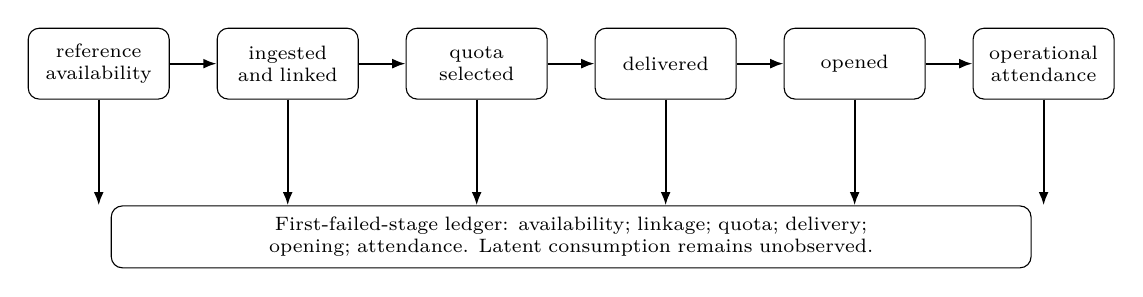
\begin{tikzpicture}[font=\scriptsize,
 stage/.style={draw,rounded corners,minimum height=9mm,align=center,inner sep=2pt,text width=1.65cm},
 arr/.style={-{Latex[length=1.7mm]},thick}]
\node[stage] (a) at (0,0) {reference availability};
\node[stage] (l) at (2.4,0) {ingested and linked};
\node[stage] (q) at (4.8,0) {quota selected};
\node[stage] (d) at (7.2,0) {delivered};
\node[stage] (o) at (9.6,0) {opened};
\node[stage] (c) at (12,0) {operational attendance};
\draw[arr] (a)--(l); \draw[arr] (l)--(q); \draw[arr] (q)--(d);
\draw[arr] (d)--(o); \draw[arr] (o)--(c);
\node[draw,rounded corners,align=center,inner sep=4pt,text width=11.4cm] (loss) at (6,-2.2)
 {First-failed-stage ledger: availability; linkage; quota; delivery; opening; attendance. Latent consumption remains unobserved.};
\draw[arr] (a)--(loss.north -| a); \draw[arr] (l)--(loss.north -| l);
\draw[arr] (q)--(loss.north -| q); \draw[arr] (d)--(loss.north -| d);
\draw[arr] (o)--(loss.north -| o); \draw[arr] (c)--(loss.north -| c);
\end{tikzpicture}
\caption{Staged omission from reference availability to operational attendance. Historical \texttt{picked} logs stop at selection.}
\label{fig:omission-stages}
\end{figure}

\subsubsection{4.3 Operational attendance and the failure-composite
endpoint}\label{operational-attendance-and-the-failure-composite-endpoint}

Before outcome unblinding, each domain must freeze an instrument
registry: instrument/version, raw-event schema, decision rule,
thresholds, validation data and code hash, measurement error,
alternative instruments, and assessor blinding. The reference executor
ships a \texttt{synthetic\_instrument\_fixture} registry object, not a
complete preregistered instrument registry; code that claims
\texttt{validated} status must carry the full registration fields---true
64-character hexadecimal validation/code hashes, sensitivity/specificity
intervals, a declared validation-to-deployment transportability
assumption, an independent blinded reference-set construction and unlock
record with no tuning/main-corpus overlap, and a completion-subset
representativeness statement---and is rejected otherwise. These are
structural registration checks, not completed measurement validation.
For digital text, the primary decision rule is
\texttt{VALID\_READING\_AND\_CONTENT\_LINKED\_CONFIRMATION}, explicitly

\[Z=1\iff \text{valid reading event}\ \mathbf{AND}\ \text{content-linked confirmation/task operation}.\]

A valid reading event requires focused visibility, engaged time, and
content coverage above frozen thresholds. Opening, dwell, click, or
scroll alone is insufficient. A complete validated measurement that
fails the conjunction is operational negative; missing, invalid, or
non-adjudicable measurement is \texttt{unknown}. Non-finite telemetry,
negative engaged time, coverage outside \([0,1]\), non-Boolean flags,
and empty evidence pointers are invalid and yield unknown, never
positive or negative; thresholds themselves are checked for finiteness
and range at registration. Human adjudicators and validation annotators
must be blind to arm, model family, and comparative outcomes. Machine
ingestion-and-task-reference is reported separately and never
substituted for human attendance.

The sole prospective primary endpoint uses \(Y^{FC}_{aj}=1\) unless
target \(j\) in arm \(a\) has a valid positive operational attendance
measurement. Its weighted form is

\[\mathcal M^{FC}_{\nu,a}=\sum_j\nu_jY^{FC}_{aj}.\tag{5}\]

Explicit abstention, observed non-attendance, and unknown terminal
outcomes all enter \(Y^{FC}=1\). This measures failure to obtain
confirmed operational attendance; it does not recover latent
\(\mathcal M_\nu\). Failure coding is conservative for an arm's omission
level but need not be conservative for a between-arm contrast.

Let
\(u_a=\sum_j\nu_j1\{\text{terminal operational outcome unknown in arm }a\}\),
and let \(\mathcal M_{\nu,a}^{Z}\) denote \textbf{operational attendance
omission} after unknown operational outcomes are assigned to success or
failure. For
\(\Delta^{FC}=\mathcal M^{FC}_{\nu,sea}-\mathcal M^{FC}_{\nu,control}\),
the sharp no-assumption bounds are

\[\Delta^{FC}-u_{sea}\ \le\ \mathcal M_{\nu,sea}^{Z}-\mathcal M_{\nu,control}^{Z}\ \le\ \Delta^{FC}+u_{control}.\tag{6}\]

These are \textbf{operational} bounds, not latent actual-consumption
bounds. The lower extreme assigns sea unknowns to operational success
and control unknowns to operational failure; the upper extreme reverses
the assignment. Both arm-specific extremes must be reported, together
with missingness by arm, stage, and reason.

They do not bound \(\mathcal M_{\nu,sea}-\mathcal M_{\nu,control}\)
without a measurement-consistency assumption. For example, with no
unknowns the operational bounds collapse to
\([\Delta^{FC},\Delta^{FC}]\), and to \([0,0]\) when additionally
\(\Delta^{FC}=0\); a SEA false positive (\(Z=1,D=0\)) and a control true
positive (\(Z=1,D=1\)) then give latent omission contrast 1. False
negatives in completed negative measurements give analogous violations.
To transport operational bounds to latent consumption, one must at least
assume that non-unknown measurements perfectly classify \(D\); otherwise
arm-specific sensitivity/specificity and their uncertainty must be
modeled. Under an explicit arm-specific error model whose rates are
conditionally stable between the validation and deployment populations,
completed-measurement omission transports by the supplement's identity
(S12), with a precision warning and an error-rate sensitivity grid when
the Youden denominator \(se_a+sp_a-1\) approaches zero. When
sensitivity, specificity, and operational omission share a validation
set, uncertainty propagation needs covariance terms or a joint (cluster)
bootstrap, not assumed independence; stratified heterogeneity and
completion-gap diagnostics support---but never prove---transportability
and completion-subset representativeness. The future protocol therefore
preregisters misclassification validation, transportability checks, and
arm-differential error comparison before outcome unlock. Best-case
coding, arm-aware inverse-probability weighting, and separately
justified multiple imputation are sensitivity analyses only.

\subsubsection{4.4 Mean intervals are not pointwise
guarantees}\label{mean-intervals-are-not-pointwise-guarantees}

A Clopper--Pearson interval can estimate a weighted mean only under
independent target--environment--evaluation units and a declared
superpopulation model (Clopper \& Pearson, 1934). It does not estimate a
uniform per-proposition floor, a maximum independent-subset size, or
simultaneous coverage across classes. On one complete finite corpus,
proportions are descriptive. The supplement gives the formal CP
statement and its limits; the main text does not use historical
run-level intervals as deployment guarantees.

\subsection{5 Conditional Technical
Foundations}\label{conditional-technical-foundations}

This section collects standard or directly inherited results used by the
framework. They are not presented as multiple new theorems. Proofs,
boundary cases, and model-calculated tables are in
\texttt{docs/SUPPLEMENT\_FORMAL\_AND\_SECONDARY\_v1.16.md}; all
retrospective selected-proxy estimates are retained only in
\texttt{docs/SUPPLEMENT\_RETROSPECTIVE\_AUDITS\_v1.16.md}, regenerated
from frozen data files.

\textbf{One update kernel.} Under integrability and attainment, expected
realized decision value can be written as

\[W(c,\hat c)=\mathrm{VOI}_c-\operatorname{Regret}_c(\hat c),\tag{7}\]

where the agent uses one assumed update kernel for every signal and
regret is evaluated under the true law. The identity follows by adding
and subtracting the correctly specified optimal action value. A binary
counterexample gives negative realized value when misspecification
regret exceeds correctly specified information value. This is a boundary
clarification, not a new general value-of-information theorem.

\textbf{Capacity and thresholds.} A minimum per-item cost gives a
capacity bound; a clairvoyant top-\(m\) oracle gives a lower bound on
leaked value, not an attainable non-anticipating policy. Population
threshold feasibility and finite top-\(m\) expected recall are different
models. For the Gaussian example in the supplement, the required
population separation is \(d'=4.389337888\) with AUC 0.999044514;
finite-pool expectations and Monte Carlo predictive quantiles are
reported separately. Neither is empirical ex-ante critical recall.

\textbf{Coverage, online choice, and budget prices.} Weighted coverage
and facility-location diversity inherit monotone-submodular guarantees
only on certified domains and for the stated algorithm variant. Online
threshold recursions require explicit boundary cases. Conditional EIG
submodularity requires joint conditional independence given the
knowledge state. Fixed-capacity KL subset choice is a subset-level
logit, not a single-item logit. Separable concave time allocation
satisfies standard KKT conditions with shadow price \(\lambda_B\); this
does not solve path-dependent retrieval--push coupling. These results
are retained because the framework needs their precise domains, not
because their count is evidence of theoretical novelty.

\section{Part II Evidence, Protocol, and
Scope}\label{part-ii-evidence-protocol-and-scope}

\subsection{6 Frozen Retrospective Sensitivity
Audits}\label{frozen-retrospective-sensitivity-audits}

\subsubsection{6.1 Authoritative evidence
matrix}\label{authoritative-evidence-matrix}

Table 4 is the single authoritative summary. ``Completed'' refers only
to the named formal, synthetic, or retrospective artifact.

\textbf{Table 4. Claim--assumption--evidence matrix.}

\begin{longtable}[]{@{}
  >{\raggedright\arraybackslash}p{(\linewidth - 6\tabcolsep) * \real{0.2500}}
  >{\raggedright\arraybackslash}p{(\linewidth - 6\tabcolsep) * \real{0.2500}}
  >{\raggedright\arraybackslash}p{(\linewidth - 6\tabcolsep) * \real{0.2500}}
  >{\raggedright\arraybackslash}p{(\linewidth - 6\tabcolsep) * \real{0.2500}}@{}}
\toprule\noalign{}
\begin{minipage}[b]{\linewidth}\raggedright
Claim or artifact
\end{minipage} & \begin{minipage}[b]{\linewidth}\raggedright
Critical assumptions
\end{minipage} & \begin{minipage}[b]{\linewidth}\raggedright
Evidence status
\end{minipage} & \begin{minipage}[b]{\linewidth}\raggedright
What is not supported
\end{minipage} \\
\midrule\noalign{}
\endhead
\bottomrule\noalign{}
\endlastfoot
Conditional SAP framework & Finite discrete model; declared target
registry and budgets & Formal specification; synthetic executor & Joint
optimality, tractability, identified utility \\
Governance reference & Structural authorization fixtures; retained
anchor & 18/18 synthetic conformance/negative tests & Authenticated
identity, malicious-host security, human control \\
Longitudinal executor & Declared synthetic fixture and instrument &
Two-period run, guard/budget/audit checks & Deployment effectiveness or
real consumption \\
Target-construction audit & Deterministic extraction rules; frozen
arbitration & Rule agreement and granularity sensitivity & Independent
human target validation \\
Weighted omission theory & Declared \(\nu\), coverage law, latent
consumption & Formal identities and bounds & Measured uniform floor or
deployment recall \\
Financial retrospective audit & Frozen rows; realized labels enter
selection & Public CSV reproduction; 7/7 budget alarms & R4-compliant
95\% delivery or independent targets \\
Four-family replay & Fixed digest; citation-proxy labels; selected only
& Three retrospective calibers and 17 scenarios & Actual consumption,
independent environments, structural benefit \\
Future matched protocol & Public preregistration; independent
environments & Design only & Any completed S2d/S4/S5 or human effect \\
\end{longtable}

\subsubsection{6.2 A representative falsification of a strong
reading}\label{a-representative-falsification-of-a-strong-reading}

The financial historical aggregate reports 120 hits over \(7\times18\)
recurring agent--target evaluations, numerically \(120/126=0.952381\). A
quick reading might treat this as crossing a 95\% target. The audit
overturns that strong reading: the seven configurations all trigger
budget-conflict alarms because inherited supply exceeds the Channel-I
cap; the denominator is recurring evaluations, not 126 independent
targets; realized legal/market labels enter the semi-oracle score; and
historical selections are frozen-row aggregates rather than
independently reconstructed runs. The public 1,260-row CSV is
hash-pinned and default reproduction verifies its bytes and row count
without reading Git history. This example shows why the paper reports
accounting boundaries rather than a benefit headline.

\subsubsection{6.3 Four-family key flow and caliber
boundaries}\label{four-family-key-flow-and-caliber-boundaries}

The frozen replay has 72,000 expected unique keys: 71,970 existing keys
and 30 no-row keys. Existing keys comprise 71,914 nonempty-selection
keys and 56 empty-only keys. There are 73,704 structurally parseable
records, including 157 empty records; 101 empty records share nonempty
keys. Historical logs cannot distinguish valid abstention from silent
execution failure. No delivered/opened/attended fields exist.

Table 5 gives the three post-hoc descriptive conventions. They answer
different data-quality questions and are not prospective primary
analyses.

\textbf{Table 5. Retrospective selected-proxy caliber populations.}

\begin{longtable}[]{@{}
  >{\raggedright\arraybackslash}p{(\linewidth - 8\tabcolsep) * \real{0.1875}}
  >{\raggedleft\arraybackslash}p{(\linewidth - 8\tabcolsep) * \real{0.2500}}
  >{\raggedright\arraybackslash}p{(\linewidth - 8\tabcolsep) * \real{0.1875}}
  >{\raggedright\arraybackslash}p{(\linewidth - 8\tabcolsep) * \real{0.1875}}
  >{\raggedright\arraybackslash}p{(\linewidth - 8\tabcolsep) * \real{0.1875}}@{}}
\toprule\noalign{}
\begin{minipage}[b]{\linewidth}\raggedright
Caliber
\end{minipage} & \begin{minipage}[b]{\linewidth}\raggedleft
Recall/return keys
\end{minipage} & \begin{minipage}[b]{\linewidth}\raggedright
No-row keys
\end{minipage} & \begin{minipage}[b]{\linewidth}\raggedright
Conflicts
\end{minipage} & \begin{minipage}[b]{\linewidth}\raggedright
Role
\end{minipage} \\
\midrule\noalign{}
\endhead
\bottomrule\noalign{}
\endlastfoot
\texttt{ALL\_EXISTING\_}\allowbreak \texttt{RECORD\_MEAN\_}\allowbreak \texttt{ZERO\_EMPTY}
& 71,970 / 71,970 & Missing & Attempt means & Designated retrospective
descriptive convention \\
\texttt{ALL\_EXPECTED\_}\allowbreak \texttt{RECORD\_MEAN\_}\allowbreak \texttt{ZERO\_EMPTY\_}\allowbreak \texttt{NO\_ROW}
& 72,000 / 72,000 & Selected-proxy zero & Attempt means & Conservative
selection-failure sensitivity \\
\texttt{METRIC\_RESOLVED\_}\allowbreak \texttt{ZERO\_EMPTY} & 71,629 /
70,732 & Missing & Metric-specific refusal & Conflict-refusing
sensitivity \\
\end{longtable}

All family point estimates, run-level ranges, standard deviations, sign
counts, bootstrap intervals, nominal tests, Rule A, strict-singleton,
17-scenario ranges, and citation-return decompositions are moved to
\texttt{docs/SUPPLEMENT\_RETROSPECTIVE\_AUDITS\_v1.16.md}. They are
exploratory descriptions on one shared 30-day corpus with retrospective
labels, upstream digest conditioning, and confounded
family/backend/prompt/runtime configurations. Run-level resampling does
not create independent environments. The main text therefore does not
use those numbers to support SEA's structural effect.

Two leakage channels remain. Retrospective proxy dependence is present
by construction: four-family digests use 2026 citation counts, and the
financial semi-oracle uses realized labels. Model memory and incomplete
point-in-time availability remain unquantified; no complete memory
ablation, post-cutoff replication, anonymized-title arm, or
pre-availability filter has been performed. Historical shards contain
zero archived call, token, fee, latency, or retry fields in the required
schema, so no retrospective efficiency advantage is inferred.

\subsection{7 A Proposed Minimum Matched
Evaluation}\label{a-proposed-minimum-matched-evaluation}

The \textbf{one primary comparison} is SEA's guarded staged pipeline
versus the same model performing end-to-end screening from the raw
candidate stream. The \textbf{one primary outcome} is the all-assigned
failure-composite weighted omission \(\mathcal M^{FC}_{\nu}\) defined in
Section 4.3. RAG with safety filtering, welfare-oriented recommendation,
decision value, efficiency, and ablations are hierarchical secondary
analyses with prespecified gatekeeping; there are not multiple primary
outcomes.

Arms must match model instance, raw inputs, retrieval permissions, index
snapshots, context/reasoning budgets, and consumption limits. At least
three nonoverlapping time windows, two domains, and one post-cutoff or
private corpus are minimum coverage requirements, not a power claim.
Power must be simulated on independent corpus/month units with
between-environment variance, within-cluster correlation, missingness,
and the primary endpoint. Agent-day multiplication is forbidden as a
substitute.

Before unlocking outcomes, the protocol must freeze the registry family,
version schedule, switch timing, and allowed reset targets (exogenous
protocol events, not policy actions), reference availability audits,
attendance instruments, thresholds, validation sets, blind adjudication,
sensitivity versions, and the arm-specific missing-outcome bounds.
Instrument validation must estimate arm-specific sensitivity and
specificity on an independent blinded reference set, check
validation-to-deployment error transportability and completion-subset
representativeness with stratified diagnostics, report the AND rule's
operational false-negative rate, and preregister an arm-differential
error comparison; the completed-measurement transport identity
(supplement S12) is a sensitivity analysis under that explicit error
model, with covariance-aware or joint-bootstrap uncertainty propagation,
a near-zero-denominator precision warning, and a pre-specified
sensitivity grid, not an assumption-free bound. A time-stamped public
registry entry must precede final-corpus unlock; an internally frozen
document is not public preregistration. The complete protocol is
\texttt{docs/MINIMAL\_VALID\_EXPERIMENT\_v1.16.md}. No human RCT is a
precondition for the present framework/artifact contribution; direct
human evidence becomes necessary only for human learning, welfare, or
transfer claims.

\subsection{8 Limitations and
Conclusion}\label{limitations-and-conclusion}

The SAP is a conditional controlled model, not a jointly solved system.
The non-composition example shows why valid component guarantees need
not compose, and Algorithm 1 has no global approximation claim. The
governance reference and longitudinal executor establish synthetic
interface conformance, not authenticated identity, malicious-host
security, meaningful human control, or deployment effectiveness.
Operational attendance is a validated behavioral measurement, not latent
comprehension; machine ingestion-and-task-reference is not human
attention.

Historical \texttt{picked} records measure selection proxies only. The
three retrospective calibers make denominator and conflict assumptions
explicit, but disclosure of non-identifiability does not turn positive
point estimates into benefit evidence. The defensible contribution is
therefore a conditional framework, a checkable governance/executor
artifact, and a falsifiable omission-audit specification. Comparative
effectiveness and human consequences remain hypotheses for the
preregistered matched protocol. Independent human mathematical review,
third-party reproduction, real matched experiments, and human data
remain pending.

\subsection{Data and Code
Availability}\label{data-and-code-availability}

The current public candidate snapshot is \textbf{\texttt{v1.16.0}},
maintained at \url{https://github.com/hurrywhen/sea-nuaa} and
\url{https://gitee.com/jiangsu-yunhefeng-intelligent_0/sea-nuaa}. Entry
points are \texttt{RELEASE\_v1.16.md},
\texttt{docs/REPRODUCIBILITY\_v1.16.md},
\texttt{sim/pilot/results/evidence\_status\_v1.16.json}, and the
versioned artifact manifest. The historical v1.7 version DOI
\url{https://doi.org/10.5281/zenodo.23620920} and concept DOI
\url{https://doi.org/10.5281/zenodo.23620919} do not cover v1.9, v1.10,
v1.11, v1.13, v1.14, v1.15, or v1.16. No v1.16-specific DOI or public
experimental preregistration is asserted without a persistent record.

The snapshot provides the governance reference and 18 tests
(\texttt{sim/sea\_governance/}), the minimal longitudinal executor and
target-construction audit (\texttt{sim/sea\_sap/}), the worked
non-composition example (\texttt{tools/reproduce\_v110\_sap.py}, stable
historical filename), retained mathematical regressions
(\texttt{tools/reproduce\_v19\_math.py}), the three retrospective
calibers and future schema
(\texttt{sim/sea\_pilot/audit\_v110\_consumption\_caliber.py}, stable
script/result paths), the single-source retrospective table generator
(\texttt{tools/make\_retrospective\_tables.py}),
financial/upstream/citation-return audits, and the unexecuted protocol
and supplements. Exact commands, dependencies, frozen-input hashes, and
clean-snapshot checks are consolidated in
\texttt{docs/REPRODUCIBILITY\_v1.16.md}. Analyses are read-only by
default; writing dedicated artifacts requires \texttt{-\/-write}, and
replacement requires \texttt{-\/-force}. The scripts make no LLM calls
and create no human data. Author-run clean-snapshot checks are not
third-party reproduction.

\subsection{Human--AI Collaboration and Responsibility
Statement}\label{humanai-collaboration-and-responsibility-statement}

AI agents assisted with literature searching, mathematical
re-derivation, code generation, numerical checks, and manuscript
drafting. Model families studied in the replay are both research
instruments and research objects; shared prompts, infrastructure,
corpora, and model biases remain conflict channels rather than
independent replications. The human authors retain responsibility for
the research question, design decisions, treatment of negative results,
authorship, and any submission decision. Computational tests and
AI-assisted proof checks are not independent human mathematical
verification. \textbf{Independent human mathematical review remains
pending.} No AI system holds approval authority over objective writes,
publication, or human-subject decisions.

\subsection{References}\label{references}

\begingroup\footnotesize

Allcott, H., Braghieri, L., Eichmeyer, S., \& Gentzkow, M. (2020). The
welfare effects of social media. \emph{American Economic Review,
110}(3), 629--676.

Bergman, O., \& Whittaker, S. (2016). \emph{The Science of Managing Our
Digital Stuff}. MIT Press.

Berk, R. H. (1966). Limiting behavior of posterior distributions when
the model is incorrect. \emph{The Annals of Mathematical Statistics,
37}(1), 51--58. https://doi.org/10.1214/aoms/1177699597

Blackwell, D. (1953). Equivalent comparisons of experiments. \emph{The
Annals of Mathematical Statistics, 24}(2), 265--272.

Carbonell, J., \& Goldstein, J. (1998). The use of MMR, diversity-based
reranking for reordering documents and producing summaries. In
\emph{Proceedings of the 21st Annual International ACM SIGIR Conference
on Research and Development in Information Retrieval} (pp.~335--336).

Chaloner, K., \& Verdinelli, I. (1995). Bayesian experimental design: A
review. \emph{Statistical Science, 10}(3), 273--304.

Charnov, E. L. (1976). Optimal foraging, the marginal value theorem.
\emph{Theoretical Population Biology, 9}(2), 129--136.

Chow, C. K. (1970). On optimum recognition error and reject tradeoff.
\emph{IEEE Transactions on Information Theory, 16}(1), 41--46.
https://doi.org/10.1109/TIT.1970.1054406

Clopper, C. J., \& Pearson, E. S. (1934). The use of confidence or
fiducial limits illustrated in the case of the binomial.
\emph{Biometrika, 26}(4), 404--413.
https://doi.org/10.1093/biomet/26.4.404

Cochran, W. G. (1954). Some methods for strengthening the common
\(\chi^2\) tests. \emph{Biometrics, 10}(4), 417--451.
https://doi.org/10.2307/3001616

Dang, V., \& Croft, W. B. (2012). Diversity by proportionality: An
election-based approach to search result diversification. In
\emph{Proceedings of the 35th International ACM SIGIR Conference on
Research and Development in Information Retrieval} (pp.~65--74).

Efron, B. (1979). Bootstrap methods: Another look at the jackknife.
\emph{The Annals of Statistics, 7}(1), 1--26.
https://doi.org/10.1214/aos/1176344552

Es, S., James, J., Espinosa Anke, L., \& Schockaert, S. (2024). RAGAs:
Automated evaluation of retrieval augmented generation. In
\emph{Proceedings of the 18th Conference of the European Chapter of the
Association for Computational Linguistics: System Demonstrations}
(pp.~150--158). https://doi.org/10.18653/v1/2024.eacl-demo.16

Esponda, I., \& Pouzo, D. (2016). Berk--Nash equilibrium: A framework
for modeling agents with misspecified models. \emph{Econometrica,
84}(3), 1093--1130.

Friedman, B., \& Hendry, D. G. (2019). \emph{Value Sensitive Design:
Shaping Technology with Moral Imagination}. MIT Press.

Fudenberg, D., Romanyuk, G., \& Strack, P. (2017). Active learning with
a misspecified prior. \emph{Theoretical Economics, 12}(3), 1155--1189.

Geifman, Y., \& El-Yaniv, R. (2017). Selective classification for deep
neural networks. In \emph{Advances in Neural Information Processing
Systems 30} (pp.~4878--4887).

Gittins, J. C. (1979). Bandit processes and dynamic allocation indices.
\emph{Journal of the Royal Statistical Society: Series B, 41}(2),
148--177.

Harper, F. M., Xu, F., Kaur, H., Condiff, K., Chang, S., \& Terveen, L.
G. (2015). Putting users in control of their recommendations. In
\emph{Proceedings of the 9th ACM Conference on Recommender Systems}
(pp.~3--10). https://doi.org/10.1145/2792838.2800179

Hirsch, T., Merced, K., Narayanan, S., Imel, Z. E., \& Atkins, D. C.
(2017). Designing contestability: Interaction design, machine learning,
and mental health. In \emph{Proceedings of the 2017 Conference on
Designing Interactive Systems} (pp.~95--99).
https://doi.org/10.1145/3064663.3064703

Jugovac, M., \& Jannach, D. (2017). Interacting with
recommenders---Overview and research directions. \emph{ACM Transactions
on Interactive Intelligent Systems, 7}(3), Article 10, 1--46.
https://doi.org/10.1145/3001837

Karush, W. (1939). \emph{Minima of Functions of Several Variables with
Inequalities as Side Conditions} {[}Master's thesis, University of
Chicago{]}. Reprinted in \emph{Traces and Emergence of Nonlinear
Programming} (2014, pp.~217--245).
https://doi.org/10.1007/978-3-0348-0439-4\_10

Krause, A., Singh, A., \& Guestrin, C. (2008). Near-optimal sensor
placements in Gaussian processes: Theory, efficient algorithms and
empirical studies. \emph{Journal of Machine Learning Research, 9},
235--284.

Kuhn, H. W., \& Tucker, A. W. (1951). Nonlinear programming. In
\emph{Proceedings of the Second Berkeley Symposium on Mathematical
Statistics and Probability} (pp.~481--492). University of California
Press. https://doi.org/10.1525/9780520411586-036

Leskovec, J., Krause, A., Guestrin, C., Faloutsos, C., VanBriesen, J.,
\& Glance, N. (2007). Cost-effective outbreak detection in networks. In
\emph{Proceedings of the 13th ACM SIGKDD International Conference on
Knowledge Discovery and Data Mining} (pp.~420--429).

Lewis, P., Perez, E., Piktus, A., Petroni, F., Karpukhin, V., Goyal, N.,
Küttler, H., Lewis, M., Yih, W.-t., Rocktäschel, T., Riedel, S., \&
Kiela, D. (2020). Retrieval-augmented generation for knowledge-intensive
NLP tasks. In \emph{Advances in Neural Information Processing Systems
33} (pp.~9459--9474).
https://proceedings.neurips.cc/paper/2020/hash/6b493230205f780e1bc26945df7481e5-Abstract.html

Lin, H., \& Bilmes, J. (2011). A class of submodular functions for
document summarization. In \emph{Proceedings of the 49th Annual Meeting
of the Association for Computational Linguistics: Human Language
Technologies} (pp.~510--520). https://aclanthology.org/P11-1052/

Lin, X., Deldjoo, Y., Dai, S., Bao, H., Ye, X., Nazary, F., Wang, W., Di
Noia, T., Xu, J., \& Chua, T.-S. (2026). Autonomous information seeking:
A roadmap for agentic recommender systems. \emph{arXiv:2607.04433v1}.
https://doi.org/10.48550/arXiv.2607.04433

Lindley, D. V. (1956). On a measure of the information provided by an
experiment. \emph{The Annals of Mathematical Statistics, 27}(4),
986--1005.

Mantel, N., \& Haenszel, W. (1959). Statistical aspects of the analysis
of data from retrospective studies of disease. \emph{Journal of the
National Cancer Institute, 22}(4), 719--748.
https://doi.org/10.1093/jnci/22.4.719

Matějka, F., \& McKay, A. (2015). Rational inattention to discrete
choices: A new foundation for the multinomial logit model.
\emph{American Economic Review, 105}(1), 272--298.

Maćkowiak, B., Matějka, F., \& Wiederholt, M. (2023). Rational
inattention: A review. \emph{Journal of Economic Literature, 61}(1),
226--273.

McNemar, Q. (1947). Note on the sampling error of the difference between
correlated proportions or percentages. \emph{Psychometrika, 12}(2),
153--157. https://doi.org/10.1007/BF02295996

Nemhauser, G. L., Wolsey, L. A., \& Fisher, M. L. (1978). An analysis of
approximations for maximizing submodular set functions---I.
\emph{Mathematical Programming, 14}, 265--274.

Papadimitriou, C. H., \& Tsitsiklis, J. N. (1999). The complexity of
optimal queueing network control. \emph{Mathematics of Operations
Research, 24}(2), 293--305.

Peng, Q., Liu, H., Huang, H., Yang, J., Yang, Q., \& Shao, M. (2025). A
survey on LLM-powered agents for recommender systems. In \emph{Findings
of the Association for Computational Linguistics: EMNLP 2025}
(pp.~11574--11583). https://doi.org/10.18653/v1/2025.findings-emnlp.620

Pielot, M., Church, K., \& de Oliveira, R. (2014). An in-situ study of
mobile phone notifications. In \emph{Proceedings of the 16th
International Conference on Human-Computer Interaction with Mobile
Devices \& Services} (pp.~43--52).

Pirolli, P., \& Card, S. K. (1999). Information foraging.
\emph{Psychological Review, 106}(4), 643--675.

Resnick, S. I. (1987). \emph{Extreme Values, Regular Variation, and
Point Processes}. Springer.

Saad-Falcon, J., Khattab, O., Potts, C., \& Zaharia, M. (2024). ARES: An
automated evaluation framework for retrieval-augmented generation
systems. In \emph{Proceedings of NAACL-HLT 2024 (Volume 1: Long Papers)}
(pp.~338--354). https://doi.org/10.18653/v1/2024.naacl-long.20

Santoni de Sio, F., \& van den Hoven, J. (2018). Meaningful human
control over autonomous systems: A philosophical account.
\emph{Frontiers in Robotics and AI, 5}, Article 15.
https://doi.org/10.3389/frobt.2018.00015

Santos, R. L. T., Macdonald, C., \& Ounis, I. (2010). Exploiting query
reformulations for web search result diversification. In
\emph{Proceedings of the 19th International Conference on World Wide
Web} (pp.~881--890). https://doi.org/10.1145/1772690.1772780

Savage, L. J. (1951). The theory of statistical decision. \emph{Journal
of the American Statistical Association, 46}(253), 55--68.
https://doi.org/10.1080/01621459.1951.10500768

Settles, B. (2009). \emph{Active Learning Literature Survey} (Computer
Sciences Technical Report 1648). University of Wisconsin--Madison.

Sims, C. A. (2003). Implications of rational inattention. \emph{Journal
of Monetary Economics, 50}(3), 665--690.

Stigler, G. J. (1961). The economics of information. \emph{Journal of
Political Economy, 69}(3), 213--225.

Stray, J., Halevy, A., Assar, P., Hadfield-Menell, D., Boutilier, C.,
Ashar, A., et al.~(2024). Building human values into recommender
systems: An interdisciplinary synthesis. \emph{ACM Transactions on
Recommender Systems, 2}(3), Article 20, 1--57.
https://doi.org/10.1145/3632297

Sviridenko, M. (2004). A note on maximizing a submodular set function
subject to a knapsack constraint. \emph{Operations Research Letters,
32}(1), 41--43.

Voorhees, E. M. (1998). Variations in relevance judgments and the
measurement of retrieval effectiveness. In \emph{Proceedings of the 21st
Annual International ACM SIGIR Conference on Research and Development in
Information Retrieval} (pp.~315--323).
https://doi.org/10.1145/290941.291017

Wang, L., Lin, J., \& Metzler, D. (2011). A cascade ranking model for
efficient ranked retrieval. In \emph{Proceedings of the 34th
International ACM SIGIR Conference on Research and Development in
Information Retrieval} (pp.~105--114).
https://doi.org/10.1145/2009916.2009934

Weitzman, M. L. (1979). Optimal search for the best alternative.
\emph{Econometrica, 47}(3), 641--654.

Whittle, P. (1988). Restless bandits: Activity allocation in a changing
world. \emph{Journal of Applied Probability, 25}(A), 287--298.

\endgroup

\subsection{Appendix A Stable
Notation}\label{appendix-a-stable-notation}

\textbf{Table 6. Stable notation and scope.}

\begin{longtable}[]{@{}
  >{\raggedright\arraybackslash}p{(\linewidth - 4\tabcolsep) * \real{0.3333}}
  >{\raggedright\arraybackslash}p{(\linewidth - 4\tabcolsep) * \real{0.3333}}
  >{\raggedright\arraybackslash}p{(\linewidth - 4\tabcolsep) * \real{0.3333}}@{}}
\toprule\noalign{}
\begin{minipage}[b]{\linewidth}\raggedright
Symbol
\end{minipage} & \begin{minipage}[b]{\linewidth}\raggedright
Meaning
\end{minipage} & \begin{minipage}[b]{\linewidth}\raggedright
Scope
\end{minipage} \\
\midrule\noalign{}
\endhead
\bottomrule\noalign{}
\endlastfoot
\(\mathcal T_v\) & Versioned candidate--target map & New version creates
new evaluation cohort; control continuity along one sealed path \\
\(\mathfrak R=\{\rho^{(v)}\}\) & Finite frozen registry family with
content hashes & Declared ex ante by the evaluation protocol; not
policy-writable \\
\(\rho_t=(v_t,E_{v_t},\mathcal T_{v_t},A^{ref}_{v_t})\) & Active frozen
target registry in state & Exogenous transition at frozen timing;
single-line control; declared full-reset exception \\
\(\mu_0\) & Initial state--observation law & Initial law; distinct from
registry symbols \(\rho_t,\rho^{(v)}\) \\
\(\nu^{(v)}\) & Version-indexed target measure & Chosen at evaluation
time per cohort; not KKT price \\
\(u_t\) & User state & Ranking input, not target map \\
\(c_e(S)\) & Union reference-coverage probability & Not independent
unless certified \\
\(\delta_e(S)\) & Latent consumption conversion & Conditional on
coverage \\
\(\mathcal M_\nu,\mathcal R_\nu\) & Weighted latent omission/recall &
Mean, not pointwise infimum \\
\(Z\) & Operational attendance measurement & Not latent comprehension;
invalid telemetry is unknown \\
\(\mathcal M^{FC}_{\nu,a}\) & Failure-composite operational omission &
Unknown coded as failure \\
\(u_a\) & Weighted unknown terminal outcomes & Used in contrast
bounds \\
\(\lambda_B\) & KKT budget shadow price & Separable concave model
only \\
\(H_t\) & Audit head hash & Domain-separated canonical body \\
\end{longtable}

\subsection{Appendix B Falsification
Map}\label{appendix-b-falsification-map}

\textbf{Table 7. Implementation and assumption falsification map.}

\begin{longtable}[]{@{}
  >{\raggedright\arraybackslash}p{(\linewidth - 4\tabcolsep) * \real{0.3333}}
  >{\raggedright\arraybackslash}p{(\linewidth - 4\tabcolsep) * \real{0.3333}}
  >{\raggedright\arraybackslash}p{(\linewidth - 4\tabcolsep) * \real{0.3333}}@{}}
\toprule\noalign{}
\begin{minipage}[b]{\linewidth}\raggedright
Claim
\end{minipage} & \begin{minipage}[b]{\linewidth}\raggedright
Falsifier
\end{minipage} & \begin{minipage}[b]{\linewidth}\raggedright
Required evidence
\end{minipage} \\
\midrule\noalign{}
\endhead
\bottomrule\noalign{}
\endlastfoot
Guarded objective control & Actor--principal mismatch accepted; reuse
accepted; rollback changes bytes & Governance negative tests and exact
hash verification \\
Protocol registry governance &
Non-family/tampered/out-of-schedule/mistimed switch or undeclared reset
accepted; declaration edited after results; sealed path reused; rollback
reverts registry & Timing/seal/reset negative tests;
rollback-independence test \\
Fixed-supply non-capture & Ranking changes when only platform variables
change & Fixed-supply counterfactual; supply-ecology separate \\
Consumption-aligned omission & Selected called consumed; unknown
silently zeroed & Stage ledger, operational instrument, FC rule \\
Target comparability & Merge/split pooled without aligned weights/events
& Versioned registry and granularity sensitivity \\
Historical benefit & Positive proxy estimate treated as structural
effect & Independent matched environments and preregistration \\
Human welfare & Machine receipt or attendance called learning & Direct
human measurement and validation \\
\end{longtable}

\end{document}
